\documentclass{beamer}

\usepackage[utf8]{inputenc}
\usepackage{graphicx}

\newtheorem{definicion}{Definición}
\newtheorem{ejemplo}{Ejemplo}


\title[Polinomio interpolador de Newton]{Polinomio interpolador de Newton}
\author[I. González, S. González]{Iciar González Alonso, Serezade González Torres}
\institute[ULL]{Universidad de La Laguna}
\date[16-05-2014]{16 de mayo de 2014}


%++++++++++++++++++++++++++++++++++++++++++++++++++++++++++++++++++++++++++++++
\usetheme{Madrid}

\definecolor {pantone254}{RGB}{122,59,122}

\definecolor {pantone3015}{RGB}{0,88,147}

\definecolor {pantone432}{RGB}{56,61,66}

\setbeamercolor*{palette primary}{use=structure, fg=white, bg=pantone254}

\setbeamercolor*{palette secondary}{use=structure, fg=white, bg=pantone3015}

\setbeamercolor*{palette tertiary}{use=structure, fg=white, bg=pantone432}

%++++++++++++++++++++++++++++++++++++++++++++++++++++++++++++++++++++++++++++++

\begin{document}

%++++++++++++++++++++++++++++++++++++++++++++++++++++++++++++++++++++++++++++++

\begin{frame}

  
  
\includegraphics[width=0.15\textwidth]{img/ullesc}
  \hspace*{7.0cm}
  
\includegraphics[width=0.16\textwidth]{img/fmatesc}
  \titlepage

  \begin{small}
    
    \begin{center}

    Facultad de Matemáticas\\
    Universidad de La Laguna

    \end{center}

  \end{small}
 
\end{frame}

%++++++++++++++++++++++++++++++++++++++++++++++++++++++++++++++++++++++++++++++

\begin{frame}

  \frametitle{Índice}

  \tableofcontents[pausesections]

\end{frame}

%++++++++++++++++++++++++++++++++++++++++++++++++++++++++++++++++++++++++++++++

\section{Motivación y objetivos}

%++++++++++++++++++++++++++++++++++++++++++++++++++++++++++++++++++++++++++++++

\begin{frame}

\frametitle{Motivación y objetivos}


Se comentará la finalidad del trabajo. Distinguiremos entre:

\begin{itemize}
\item
Objetivo principal: implementación con Python de las series de potencias de Newton. Concretamente hemos trabajado con dicho programa para aproximar a través de este método el valor de la función $f(x)=e^x$.
\pause  

\item
Objetivos específicos: aprender a utilizar el método de Newton para aproximar funciones a través de series de potencias, centrándonos en la aproximación de la función nombrada anteriormente.


\end{itemize}
\end{frame}

%++++++++++++++++++++++++++++++++++++++++++++++++++++++++++++++++++++++++++++++
\section{Fundamentos teóricos}

%++++++++++++++++++++++++++++++++++++++++++++++++++++++++++++++++++++++++++++++

\begin{frame}

\frametitle{Fundamentos teóricos}

En este capítulo se pasará a desarrollar de forma teórica el tema a tratar.

\begin{itemize}
\item
Historia.
\pause

\item
Teorema.

\end {itemize}
\end{frame}
%++++++++++++++++++++++++++++++++++++++++++++++++++++++++++++++++++++++++++++++

\subsection{Historia}

%++++++++++++++++++++++++++++++++++++++++++++++++++++++++++++++++++++++++++++++

\begin{frame}

\frametitle{Historia}


 \begin{definicion}
 
 La serie de potencias de Newton se trata de un teorema descubierto hacia 1664-1665 como se puede deducir, fue desarrollado por Isaac Newton. 
El descubrimiento de la generalización de la serie binómica
fue un gran resultado en sí mismo, pero además este desencadenó nuevos estudios. Este teorema fue publicado por Wallis en 1685, pero este atribuyó el descubrimiento a Newton.

  \end{definicion}



\end{frame}
%++++++++++++++++++++++++++++++++++++++++++++++++++++++++++++++++++++++++++++++

\subsection{Teorema}

%++++++++++++++++++++++++++++++++++++++++++++++++++++++++++++++++++++++++++++++

\begin{frame}

\frametitle{Teorema}


 \begin{definicion}
 
 La forma general del polinomio interpolante de Newton para $n+1$ datos 
  
$(x_0, f(x_0)), (x_1, f(x_1)),..., (x_n, f(x_n))$ es:
\[P_n(x)=a_0 + a_1(x-x_0) + a_2(x-x_0)(x-x_1) + a_3(x-X_0)(x-x_1)(x-x_2) +...\]
\[+ a_n(x-X_0)(x-x_1)(x-x_2)....(x-x_{n-1})\]

Los coeficientes $a_i$ se obtienen calculando un conjunto de cantidades denominadas diferencias divididas.
La notación para las diferencias divididas de una función f(x) están dadas por: 

\[f[x_i,x_{i+1},x_{i+2},...,x_{i+j-1},x_{i+j}]=\frac{f[x_{i+1},x_{i+2},...,x_{i+j}]-f[x_i,x_{i+1},...,x_{i+j-1}]}{x_{i+j}-x_i}\]

  \end{definicion}

\end{frame}
%++++++++++++++++++++++++++++++++++++++++++++++++++++++++++++++++++++++++++++++

\section{Procedimiento experimental}

%++++++++++++++++++++++++++++++++++++++++++++++++++++++++++++++++++++++++++++++

\begin{frame}

\frametitle{Procedimiento experimental}

\begin{definicion}

A continuación se enumerará y se desarrollarán los pasos que se han seguido en la elaboración del programa de las series de Newton en Python.

\begin{itemize}
\item
Descripción de los experimentos.
\pause

\item
Resultados obtenidos.
\pause

\item
Análisis de los resultados

\end {itemize}

\end{definicion}

\end{frame}

%++++++++++++++++++++++++++++++++++++++++++++++++++++++++++++++++++++++++++++++

\subsection{Descripción de los experimentos}

\begin{frame}

\frametitle{Descripción de los experimentos}

\begin{enumerate}

\item
Función del experimento: $f(x) = e ^ x$
\pause

\item
Intervalo del experimento: [0,1]
\pause

\item
Nodos equidistantes: 0.00, 0.25, 0.50, 0.75, 1.00
\pause

\item
Valor x = 0.43

\end{enumerate}
\end{frame}

\subsection{Resultados obtenidos}

\begin{frame}

\frametitle{Resultados obtenidos}

\begin{table}[!ht]
\begin{center}
\begin{tabular}{|c|c|c|c|} 
\hline
x & f(x) & Coeficientes & Parte literal\\ \hline
0.0 & 1.0 & 1.0 & 1.0  \\ \hline
0.25 & 1.2840254166877414 & 1.1361016667509656 & 0.43 \\ \hline
0.5 & 1.6487212707001282 & 0.6453634985971632 & 0.0774  \\ \hline
0.75 & 2.117000016612675 & 0.12219975773607672 & -0.005418  \\ \hline
1.0 & 2.718281828459045 & 0.026030877832598165 & 0.00173376\\ \hline


\end{tabular}
\end{center}
\caption{Datos y resultados del programa}
\label{tab}
\end{table}
\end{frame}

\subsection{Análisis de los resultados}

\begin{frame}

\frametitle{Análisis de los resultados}
\begin{definicion}

En el intervalo [0,1], tomando los nodos $x_0 = 0$, $x_1 = 0.25$, $x_2 = 0.5$, $x_3 = 0.75$, $x_4 = 1$, $f(0.43) = 1.53785$ y el valor del polinomio en x = 0.43 es 1.53725. Con lo cual, se comete un error de $6{x}10 ^ {-4}$.
El número de nodos ha de ser directamente proporcional al tamaño del intervalo.

\end{definicion}

\end{frame}

%+++++++++++++++++++++++++++++++++++++++++++++++++++++++++++++++++++++++++++++
\section{Conclusiones}

%++++++++++++++++++++++++++++++++++++++++++++++++++++++++++++++++++++++++++++++

\begin{frame}

\frametitle{Conclusiones}
\begin{enumerate}
\item Obtención de la aproximación de la función $f(x) = e ^ x$ mediante el polinomio de Newton implementado en Python.
\item Mejora del conocimiento en las estructuras iterativas de programación.
\item Cálculo del error cometido por el programa.
\item Aprender a aproximar funciones a través de las series de potencias.
\item Profundizar en los fundamentos teóricos del método.

\end {enumerate}

\end{frame}
%++++++++++++++++++++++++++++++++++++++++++++++++++++++++++++++++++++++++++++++
\section{Apéndice 1. Programa Python}

%++++++++++++++++++++++++++++++++++++++++++++++++++++++++++++++++++++++++++++++

\begin{frame}

\frametitle{Apéndice 1. Programa Python}
\begin{definicion}

En este capítulo se pasará a mostrar el código mediante el cual se implemento el polinomio de Newton para la funcion $f(x)=e ^ x$.
\end {definicion}

\end{frame}
%++++++++++++++++++++++++++++++++++++++++++++++++++++++++++++++++++++++++++++++
\subsection{Almacenamiento de x}

%++++++++++++++++++++++++++++++++++++++++++++++++++++++++++++++++++++++++++++++

\begin{frame}

\frametitle{Almacenamiento de x}
\begin{center}
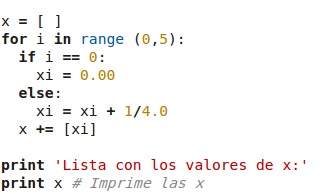
\includegraphics[width=0.75\textwidth]{img/x}
\end{center}
\end{frame}
%++++++++++++++++++++++++++++++++++++++++++++++++++++++++++++++++++++++++++++++

\subsection{Almacenamiento de f(x)}

%++++++++++++++++++++++++++++++++++++++++++++++++++++++++++++++++++++++++++++++

\begin{frame}

\frametitle{Almacenamiento de f(x)}
\begin{center}
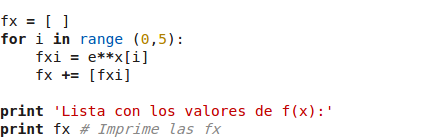
\includegraphics[width=0.75\textwidth]{img/y}
\end{center}
\end{frame}
%++++++++++++++++++++++++++++++++++++++++++++++++++++++++++++++++++++++++++++++

\subsection{Coeficientes}

%++++++++++++++++++++++++++++++++++++++++++++++++++++++++++++++++++++++++++++++



\begin{frame}

\frametitle{Coeficientes}
\begin{center}
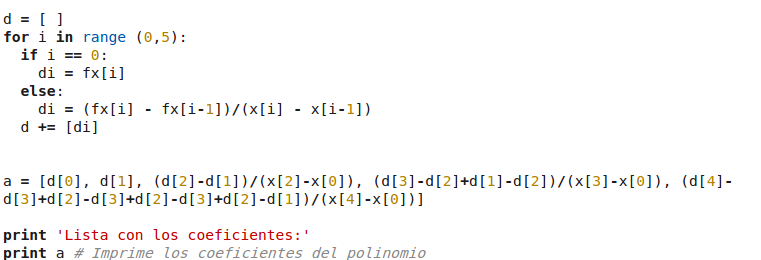
\includegraphics[width=1\textwidth]{img/coef}
\end{center}
\end{frame}


%++++++++++++++++++++++++++++++++++++++++++++++++++++++++++++++++++++++++++++++

\subsection{Partes literales del polinomio}

%++++++++++++++++++++++++++++++++++++++++++++++++++++++++++++++++++++++++++++++


\begin{frame}

\frametitle{Partes literales}
\begin{center}
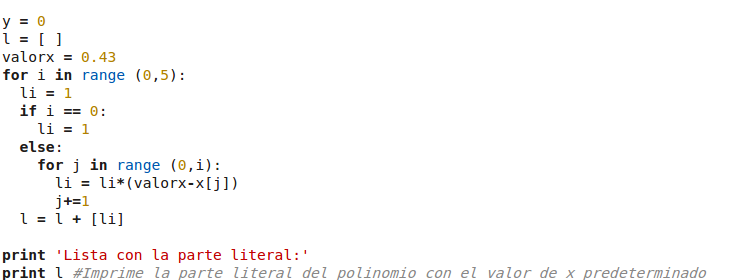
\includegraphics[width=1\textwidth]{img/lit}
\end{center}
\end{frame}
%+++++++++++++++++++++++++++++++++++++++++++++++++++++++++++++++++++++++++++++

\subsection{Valores}

%++++++++++++++++++++++++++++++++++++++++++++++++++++++++++++++++++++++++++++++


\begin{frame}

\frametitle{Valores}
\begin{center}
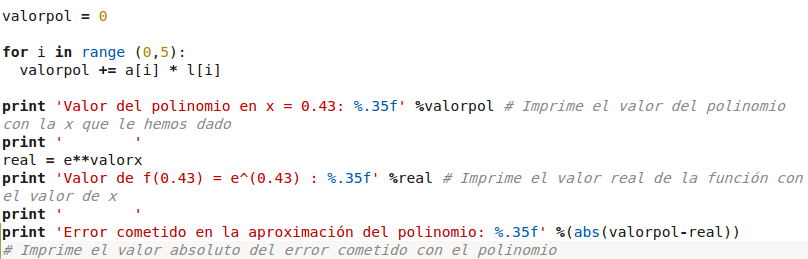
\includegraphics[width=1\textwidth]{img/val}
\end{center}
\end{frame}
%+++++++++++++++++++++++++++++++++++++++++++++++++++++++++++++++++++++++++++++
\section{Bibliografía}

%++++++++++++++++++++++++++++++++++++++++++++++++++++++++++++++++++++++++++++++
\begin{frame}
  \frametitle{Bibliografía}

\begin{thebibliography}{1}

\bibitem{python}"Solo Ciencia". http://www.solociencia.com/cientificos/isaac-newton-teorema-binomio.htm
\bibitem{python}"ULPGC Informática". http://numat.net/tutor/newton.pdf
\bibitem{python}"Universidad Politécnica de Madrid".http://ocw.upm.es/matematica-aplicada/programacion-y-metodos-numericos/contenidos/TEMA\_3/Apuntes/InterpolacionOCW.pdf
\bibitem{python}"Instituto Tecnológico de Tuxtla Gutiérrez". https://sites.google.com/site/danaly7/unidad-5/polinomio-de-interpolacion-de-newton
\bibitem{python}"Purificación González". ETSI Bilbao"http://www.ehu.es/pegonzalez/I.Teleco/Apuntes/tema5.pdf
\end{thebibliography}

\bibliography{bibliografia}

\nocite{*}

\end{frame}

%++++++++++++++++++++++++++++++++++++++++++++++++++++++++++++++++++++++++++++++
\end{document}





















